% =====================================================================
%  CoNaIISI 2026 --- Trabajos Estudiantiles --- versión ciega para evaluación
%  Formato: A4, márgenes 2,5 cm, dos columnas de igual ancho separadas 1 cm,
%  Times 12 en el cuerpo, 10 en abstract/palabras clave/referencias, sin
%  numeración de página. Compilar: `python3 make_bib.py && latexmk` dentro de conaiisi2026/.
% =====================================================================
\documentclass[12pt,a4paper,twocolumn]{article}

\usepackage{iftex}
\ifLuaTeX
  \usepackage{fontspec}
  % Times New Roman no está instalada; TeX Gyre Termes es su clon métrico.
  \setmainfont{TeX Gyre Termes}
\else
  \usepackage[utf8]{inputenc}
  \usepackage[T1]{fontenc}
  \usepackage{times}
\fi

\usepackage[spanish,es-tabla,es-noindentfirst]{babel}
\usepackage[a4paper,margin=2.5cm,columnsep=1cm]{geometry}
\usepackage[numbers,square,sort&compress]{natbib}
\usepackage{graphicx}
\usepackage{booktabs}
\usepackage{tabularx}
\usepackage{xcolor}
\usepackage{caption}
\usepackage{url}
\usepackage[hidelinks]{hyperref}

\graphicspath{{../}}
\pagestyle{empty}
\setlength{\parskip}{0pt}
\setlength{\parindent}{0.5cm}

% Títulos de sección: Times 12 negrita, sin numerar (como en la plantilla).
\makeatletter
\renewcommand\section{\@startsection{section}{1}{\z@}%
  {-1.2ex \@plus -0.5ex \@minus -0.2ex}{0.6ex \@plus 0.2ex}%
  {\normalfont\normalsize\bfseries}}
\renewcommand\subsection{\@startsection{subsection}{2}{\z@}%
  {-1.0ex \@plus -0.4ex \@minus -0.2ex}{0.4ex \@plus 0.2ex}%
  {\normalfont\normalsize\bfseries\itshape}}
\makeatother
\setcounter{secnumdepth}{0}

% Captions: Times 10 cursiva (tablas y figuras).
\captionsetup{font={small,it},labelfont={small,it},labelsep=period,justification=centering}

% Notas al pie en 9 pt.
\renewcommand\footnotesize{\fontsize{9}{11}\selectfont}

% Marcadores de responsabilidades [A]--[F], como en la tesina.
\colorlet{respcolor}{red}
\newcommand{\resp}[1]{\textcolor{respcolor}{[#1]}}

\begin{document}

% ---------------------------------------------------------------------
%  Cabecera (versión ciega: la sección Autores queda en blanco)
% ---------------------------------------------------------------------
\twocolumn[%
  \begin{center}
    {\fontsize{16}{19}\selectfont\bfseries
      Un framework de Tubos y Filtros para el análisis de noticias de portales digitales mediante inteligencia artificial generativa\par}
    \vspace{0.4cm}
    {\fontsize{14}{17}\selectfont\bfseries \phantom{Apellido, Nombre}\par}
    {\fontsize{12}{14}\selectfont\bfseries\itshape \phantom{Universidad de origen, Unidad académica}\par}
    \vspace{0.6cm}
  \end{center}
]

% ---------------------------------------------------------------------
%  Abstract y palabras clave (Times 10)
% ---------------------------------------------------------------------
{\fontsize{10}{12}\selectfont
\noindent\textbf{Abstract}\par
\noindent\textit{El análisis de noticias de portales digitales enfrenta dos obstáculos: los atributos relevantes del discurso residen en una infraestructura inaccesible a la observación directa, y el volumen del material excede la capacidad de lectura de los investigadores. Los modelos generativos de lenguaje ofrecen una capacidad interpretativa que las técnicas previas de procesamiento de lenguaje natural no alcanzan, pero su uso en investigación social exige trazabilidad, control editorial y reproducibilidad, dimensiones que los prototipos existentes no resuelven de manera integral. Este trabajo presenta un framework que organiza el ciclo de análisis como un sistema de Tubos y Filtros: siete filtros encadenados por tubos tipados transforman el flujo de los portales en un resultado consolidado, con un repositorio común que persiste cada registro intermedio y sintonizadores por los que el experto del dominio parametriza el análisis sin intervenir en el flujo de datos. Los contratos de datos entre etapas definen un grafo de procedencia que permite reconstruir, desde cualquier resultado, las noticias, prompts y configuraciones que lo produjeron. Un filtro de verificación juzga la fidelidad de cada análisis a su evidencia y la cuantifica sin suprimir contenido, dejando la decisión editorial en manos del experto. El framework se realizó como módulo de una plataforma de gestión de código abierto sobre una infraestructura de extracción preexistente y se ejercitó de extremo a extremo sobre un corpus real de prensa regional. Se discuten sus limitaciones y las líneas de trabajo que abren.}\par
\vspace{0.5em}
\noindent\textbf{Palabras Clave}\par
\noindent Inteligencia artificial generativa, modelos de lenguaje, Tubos y Filtros, procedencia de datos, agenda-setting, análisis de noticias.\par
}
\vspace{0.8em}

% ---------------------------------------------------------------------
\section{Introducción}
% ---------------------------------------------------------------------

Los medios masivos producen la realidad social que conocemos \cite{luhmann2000} y transfieren al público la prominencia de los temas y también la de sus atributos \cite{mccombs:1972,mccombs:1997}, mecanismo que la noción de encuadre precisa \cite{entman:1993}. En la sociedad hipermediatizada \cite{carlon:2020,couldry:2017}, los atributos sustanciales de los discursos residen en una infraestructura inaccesible a la observación directa, y su volumen demanda análisis inabordables sin herramientas computacionales \cite{berry:2011}. Las técnicas de procesamiento de lenguaje natural anteriores a la arquitectura \textit{Transformer} \cite{vaswani:2017} muestran limitaciones para capturar los funcionamientos discursivos que el análisis social requiere \cite{gindin:2018}; los modelos generativos de lenguaje ofrecen una capacidad interpretativa superior \cite{pavlyshenko2024,milbauer2023}, pero su uso en investigación plantea exigencias propias.

Una revisión sistemática de la literatura identificó un patrón consolidado ---extracción por \textit{scraping}, representación por \textit{embeddings} e inferencia con modelos de lenguaje--- y cinco brechas que ningún sistema relevado resuelve de manera integral: falta de trazabilidad entre la evidencia extraída y las afirmaciones generadas, escasa calibración de la incertidumbre, carencia de gobernanza editorial con intervención humana, fragilidad de la extracción ante cambios en los portales y ausencia de esquemas de anotación comparables entre plataformas.

Este trabajo propone un framework que automatiza el análisis de noticias de portales digitales mediante inteligencia artificial generativa (IAG) bajo tres garantías: trazabilidad del flujo de datos, control editorial del experto del dominio y reproducibilidad del proceso analítico. Se desarrolla en el marco de una tesina de grado en curso en ciencias de la computación, y presenta su aporte central: la caracterización del ciclo de análisis como un sistema de Tubos y Filtros \cite{garlanshaw:1994}, cuyas propiedades se ponen al servicio de esas garantías.

% ---------------------------------------------------------------------
\section{El framework como sistema de Tubos y Filtros}
% ---------------------------------------------------------------------

En el estilo de Tubos y Filtros, los \textit{filtros} son unidades de procesamiento independientes que reciben datos por puertos de entrada y los producen por puertos de salida, y los \textit{tubos} los transportan de un puerto a otro preservando su orden \cite{garlanshaw:1994,cristia:2025}. Cuatro invariantes lo definen: ningún filtro conoce a los demás, ninguno depende del estado interno de otro, la corrección de la salida no depende del orden de los cálculos individuales, y los tubos no alteran lo que transmiten \cite{cristia:2025}. De ellos se desprenden dos consecuencias que responden a las brechas relevadas: la \textit{sustituibilidad} de cada filtro atiende a la fragilidad de la extracción y a la necesidad de reemplazar modelos accesibles por API sin reescribir el resto, y la \textit{auditabilidad lineal} responde a la brecha de trazabilidad, pues cada transformación queda localizada en un filtro identificable. Una tercera propiedad, estructural, el \textit{cierre composicional} ---un sistema entero es a su vez un filtro---, habilita recombinar etapas para distintos casos de estudio.

La Figura~\ref{fig:pipeline} resume la configuración: un \textit{pipeline} lineal de siete filtros desde la fuente ---los portales monitoreados--- hasta el sumidero ---la capa de presentación---. El diseño adopta dos especializaciones canónicas, \textit{pipeline} y \textit{tubos tipados} \cite{garlanshaw:1994}, y dos deformaciones documentadas en el catálogo de Cristiá y Pomponio \cite{cristia:2025}: un repositorio común y sintonizadores.

\begin{figure*}[t]
  \centering
  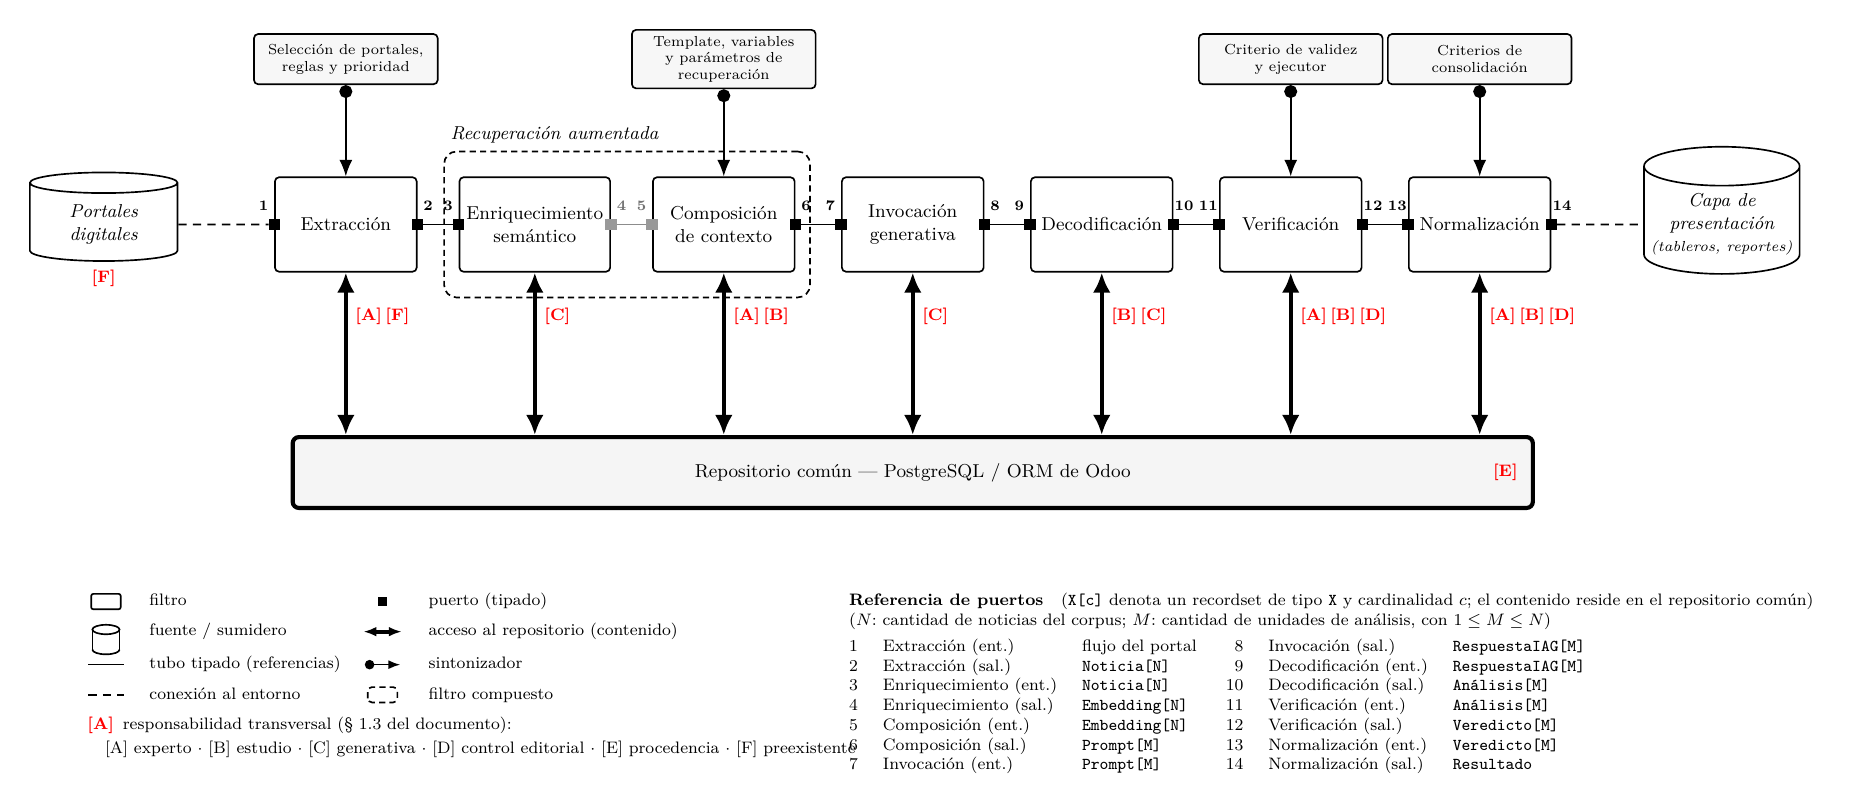
\includegraphics[width=\textwidth]{Diagrama-Arquitectura.png}
  \caption{El framework como sistema de Tubos y Filtros. Conexiones al entorno en línea discontinua, tubos en línea continua, sintonizadores con flecha originada en un círculo y acceso al repositorio con flecha bidireccional. El recuadro discontinuo agrupa Enriquecimiento semántico y Composición de contexto en el filtro compuesto Recuperación aumentada. Los marcadores en rojo señalan las responsabilidades transversales: \resp{A} intervención del experto, \resp{B} independencia del estudio, \resp{C} frontera generativa, \resp{D} control editorial, \resp{E} procedencia, \resp{F} infraestructura preexistente.}
  \label{fig:pipeline}
\end{figure*}

\subsection{Filtros y tubos tipados}

\textit{Extracción} recorre los portales registrados mediante \textit{web scraping}, recupera las publicaciones que satisfacen las reglas configuradas y persiste cada una como un registro \texttt{Noticia}; es el único filtro activo, disparado periódicamente. \textit{Enriquecimiento semántico} computa la representación vectorial de cada noticia. \textit{Composición de contexto} recupera por similitud las noticias relevantes y las integra con la plantilla de \textit{prompt}, las variables de contexto y las aclaraciones del experto; juntos implementan la generación aumentada por recuperación \cite{lewis:2020}. \textit{Invocación generativa} ejecuta cada petición contra el servicio generativo y persiste la respuesta cruda; es el filtro cuyo único cometido es esa interacción. \textit{Decodificación} valida esa respuesta contra el esquema declarado por la plantilla del estudio y la canonicaliza como \texttt{Análisis}; opera como compuerta: lo que no conforma el esquema no sigue. \textit{Verificación} contrasta cada análisis con su evidencia y emite un \texttt{Veredicto}. \textit{Normalización} consolida los veredictos en un único \texttt{Resultado} mediante una agregación determinística que cruza las claves del esquema contra una variable de comparación definida por el experto.

Cada tubo declara el tipo y la cardinalidad del \textit{recordset} que transporta, con la firma \(T[c]\): \(T\) es el tipo de los registros y \(c\) cuántos referencia. Extracción emite \texttt{Noticia[N]}; Enriquecimiento preserva \(N\); Composición redefine la cardinalidad en \(M\) unidades de análisis, con \(1 \le M \le N\), desde un único \textit{prompt} agregado hasta uno por noticia; las tres etapas siguientes preservan \(M\), como un \textit{map} sobre las unidades; y Normalización reduce a un resultado único, el \textit{reduce} que clausura el ciclo y permite escalar a corpus que no caben en una invocación del modelo.

\subsection{Repositorio común y paso por referencia}

Por los tubos no circula el contenido de las noticias, los \textit{prompts} o los análisis, sino referencias a registros que residen en un repositorio común del que todos los filtros leen y sobre el que escriben lo que producen: el patrón \textit{Claim Check} \cite{hohpe:2003}. El catálogo describe un filtro como una función de sus puertos de entrada en sus puertos de salida, \(F : \Gamma^n \to \Gamma^m\), con \(n\) y \(m\) puertos \cite{cristia:2025}; en un \textit{pipeline} de tubos tipados hay un puerto de cada lado y el dato de cada uno es un \textit{recordset}, de modo que la firma se reduce a \(f : T[c] \to T'[c']\). Aquí, además, la transformación del contenido ocurre en el repositorio, así que el estado que se transforma es el par flujo--repositorio: \(f : (T[c], \mathit{Rep}) \to (T'[c'], \mathit{Rep} \cup \Delta_f)\), donde \(\mathit{Rep}\) es el estado del repositorio al activarse el filtro y \(\Delta_f\) el conjunto de registros que éste persiste; el \textit{recordset} emitido es el conjunto de referencias a ese delta, y no su contenido. De aquí se sigue la \textit{monotonía} del repositorio: ningún filtro modifica ni elimina lo que otro produjo, condición de la trazabilidad extremo a extremo. El repositorio no compromete los invariantes ---es un almacén externo, no el estado de un filtro--- y configura una arquitectura heterogénea \cite{garlanshaw:1994}.

\subsection{Sintonizadores y plantillas de \textit{prompt}}

La intervención del experto se modela con \textit{sintonizadores}: procedimientos que un filtro expone para que la capa de presentación ajuste su comportamiento sin participar del flujo de datos \cite{cristia:2025}, equivalentes a la interfaz de control de la formulación seminal \cite{garlanshaw:1994}. Lo exponen los cuatro filtros que dependen de decisiones de dominio: Extracción (portales, reglas, prioridad), Composición (plantilla, variables, texto libre, parámetros de recuperación y del modelo), Verificación (criterio de validez y ejecutor) y Normalización (política sobre los análisis observados, variable de comparación, claves a consolidar). Los tres restantes tienen configuración técnica del implementador: el experto controla el estudio sin conocer el proveedor, y viceversa.

El sintonizador central es el de Composición, realizado sobre un panel de plantillas de \textit{prompt}. Cada plantilla declara el objetivo del análisis, las instrucciones parametrizadas con variables y el esquema de la respuesta esperada, contra el cual valida Decodificación; separar la plantilla persistente de los valores ligados por corrida sigue la práctica recomendada de la ingeniería de \textit{prompts} \cite{prompt-eng:2024}, y partir de una plantilla evita el ``síndrome de la página en blanco'' de los usuarios no expertos \cite{zamfirescu2023}. El framework no conoce el estudio: tema, pregunta, esquema y criterios ingresan como datos, no como código.

\subsection{Verificación como compuerta blanda}

El \texttt{Veredicto} asocia a cada análisis un estado ---válido, observado o no sustentado---, una medida de confianza y el sustento: los fragmentos de evidencia que respaldan o contradicen cada afirmación. Ningún análisis se suprime: los que no superan el criterio se marcan y se propagan señalados, de modo que la decisión editorial última quede en manos del analista. Esta política responde a las brechas de fidelidad, calibración de la incertidumbre \cite{pavlyshenko2024} y gobernanza editorial. El filtro es agnóstico respecto del ejecutor: un revisor humano asistido o un modelo que confronta el análisis con su evidencia (\textit{LLM-as-a-judge} \cite{zheng:2023}).

\subsection{Contratos de datos y grafo de procedencia}

Los siete tipos se especifican como contratos independientes de la plataforma bajo tres criterios: cada tipo contiene sólo la carga útil que algún filtro posterior consume y la procedencia del dato; la procedencia viaja pero la identidad del productor no ---\texttt{Embedding} no registra qué modelo computó el vector ni \texttt{RespuestaIAG} qué proveedor respondió, porque cambiar ese recurso es sustituir el filtro---; y los esquemas de dominio se delegan al estudio: en \texttt{Análisis} y \texttt{Resultado} el framework fija el sobre y la plantilla declara el contenido. Leídas en conjunto, las claves de procedencia definen sobre el repositorio un grafo de procedencia en el sentido del modelo PROV del W3C \cite{provdm:2013}: cada registro apunta a aquellos de los que se derivó, y reconstruir el origen de un resultado es una consulta de alcanzabilidad hacia atrás \cite{cuevasvicenttin:2012} que llega, desde el \texttt{Resultado}, hasta el portal, la fecha y las reglas de extracción de cada noticia que intervino.

% ---------------------------------------------------------------------
\section{El estudio como instancia del pipeline}
% ---------------------------------------------------------------------

El pipeline caracteriza el estilo; el \textit{estudio} es su instancia: fija qué \textit{recordset} ocupa cada tubo, con qué sintonizadores se invocó cada filtro, en qué etapa está la corrida y qué configuración técnica regía. El experto crea un estudio, selecciona su corpus, sintoniza los filtros, ejecuta el pipeline y lee el resultado. Cada etapa persiste su delta antes de avanzar, y una corrida interrumpida se reanuda desde ahí. La iteración del experto no reintroduce ciclos: es un estudio nuevo enlazado al anterior, que hereda su configuración y vuelve a recorrer la red. El estudio conserva así la procedencia que el grafo de tipos no cubre: con qué configuración y cuándo se produjo cada resultado. Seis responsabilidades transversales, \resp{A} a \resp{F}, siguen cada garantía hasta donde se cumple.

% ---------------------------------------------------------------------
\section{Realización y caso de aplicación}
% ---------------------------------------------------------------------

El framework se realizó, como producto de la tesina en curso, como módulo \textit{addon} de Odoo Community sobre una infraestructura institucional preexistente de extracción de noticias \cite{raimondo:2024}, de la que reutiliza sin modificación el filtro de Extracción, el modelo de datos de las publicaciones y la base de datos que oficia de repositorio común; el resto del sistema depende del extractor a través del contrato \texttt{Noticia}. Cada filtro es sustituible por herencia, las claves de procedencia son relaciones con restricción de borrado, el acceso a los modelos se aísla en un servicio con adaptadores intercambiables y pruebas automatizadas ejercitan cada garantía.

El caso de aplicación ejercitó los siete filtros de extremo a extremo sobre un corpus real: las publicaciones que la regla léxica sobre narcotráfico del extractor institucional recolectó, de un conjunto curado de portales nacionales, rosarinos y del interior de Santa Fe, durante la primera quincena de abril de 2024, en el pico de la crisis de violencia en Rosario y en el tramo en que esa regla conserva su precisión. La pregunta, propia del segundo nivel del \textit{agenda-setting}, fue con qué atributos ---localización, subtema, funciones del encuadre, actores y tono hacia la gestión provincial--- cada tipo de prensa cubre una misma cuestión. El experto declaró el estudio íntegramente como datos: una plantilla con el esquema de atributos, una estrategia de un análisis por noticia, un umbral de similitud semántica ---fijado por el presupuesto de cómputo--- para depurar el ruido de la regla léxica sin tocar el extractor, un criterio de validez explícito y la consolidación por portal, colapsada luego a tipo de prensa con una tabla de asignación publicada junto al estudio. La corrida empleó un modelo de pesos abiertos de tres mil millones de parámetros servido localmente sobre CPU, con salida estructurada, y el mismo modelo como juez. Desde el resultado consolidado puede reconstruirse el conjunto de veredictos, análisis, respuestas, \textit{prompts} y noticias que produjo cada distribución. Los resultados sustantivos se encuentran en evaluación y serán objeto de un trabajo posterior.

% ---------------------------------------------------------------------
\section{Trabajos relacionados}
% ---------------------------------------------------------------------

Los estudios de la revisión sistemática convergen en el patrón extracción, \textit{embeddings} e inferencia con modelos de lenguaje, con énfasis distintos: deduplicación semántica y agregación \cite{behbahanian}, clustering temático y publicación automatizada \cite{neupane2025}, medición de sesgo y encuadre a escala \cite{haider2025}, verificación de evidencia entre documentos \cite{milbauer2023} y cuantificación de la incertidumbre de la IAG \cite{pavlyshenko2024}. Ninguno completa el patrón con contratos de datos, procedencia de extremo a extremo, verificación editorial calibrada y plantillas gestionadas. Un antecedente metodológico cercano es Rey-Mazón \cite{mazon:2023}, que mide el \textit{agenda-setting} reconstruyendo flujos de noticias por \textit{scraping} horario.

% ---------------------------------------------------------------------
\section{Conclusión y trabajos futuros}
% ---------------------------------------------------------------------

Este trabajo caracteriza el análisis de noticias mediante IAG como un sistema de Tubos y Filtros y muestra que las propiedades del estilo se convierten en las garantías que la investigación social exige. Primero, los siete filtros con tubos tipados y repositorio común hacen sustituible cada etapa: el extractor y los proveedores de modelos quedan aislados detrás de contratos de datos. Segundo, esos mismos contratos definen un grafo de procedencia que permite reconstruir, desde cualquier resultado, las noticias, \textit{prompts} y configuraciones que lo produjeron. Tercero, los sintonizadores y las plantillas de \textit{prompt} ponen toda decisión de dominio en manos del experto y fuera del código: el framework no conoce el estudio. Cuarto, la verificación como compuerta blanda entrega un juicio de fidelidad con evidencia y confianza sin decidir por el experto.

La realización como módulo de Odoo sobre una infraestructura institucional preexistente y la corrida completa sobre un corpus real de prensa regional muestran que el diseño no es sólo descriptivo: el ciclo entero se ejecuta con un modelo local de pocos miles de millones de parámetros y deja persistida la historia íntegra de la corrida.

El diseño tiene límites conocidos: opera por lotes y no sobre un \textit{stream}, el repositorio lo acopla a la plataforma de persistencia, y la verificación con un juez del mismo modelo exhibe la etapa pero no reemplaza un control de calidad independiente. Los trabajos futuros atienden esos límites: un patrón de codificación humana para medir el acuerdo con el modelo y calibrar la confianza de los veredictos, un ejecutor de verificación independiente, y el análisis de los resultados sustantivos del caso frente a las hipótesis del \textit{agenda-setting} de segundo nivel.

% ---------------------------------------------------------------------
%  Agradecimientos, referencias y contacto (Times 10)
% ---------------------------------------------------------------------
{\fontsize{10}{12}\selectfont
\section*{Agradecimientos}
\noindent\textit{(Se completan en la versión final, con nombres y apellidos de los docentes tutores.)}
}

{\fontsize{10}{12}\selectfont
\renewcommand{\refname}{Referencias}
\bibliographystyle{unsrt}
\bibliography{refs-paper}
}

{\fontsize{10}{12}\selectfont
\section*{Datos de Contacto}
\noindent\textit{(Se completan en la versión final.)}
}

\end{document}
